\documentclass[11pt]{article}
\usepackage{algorithm2e}
\usepackage[italian]{babel}
\usepackage{ragged2e}
\usepackage{amsfonts, amssymb, amsmath}
\usepackage{cancel}
\usepackage{float}
\usepackage{mathtools}
\usepackage{hyperref}
\usepackage{subfig}
\usepackage[margin={3cm, 1.5cm}, includefoot]{geometry}
\justifying

\hypersetup{
    colorlinks=true,
    linkcolor=black,
    filecolor=black,      
    urlcolor=black,
}

\tolerance=1
\emergencystretch=\maxdimen
\hyphenpenalty=10000
\hbadness=10000

\begin{document}
\begin{titlepage}
    \begin{center}
        \vspace*{3.0cm}
            
        \Huge
        \textbf{Map Connectivity}
            
        \vspace{0.3cm}
        \LARGE
        Relazione progetto

        \vspace{1.5cm}
          
        \begin{minipage}[t]{0.47\textwidth}
            \begin{center}
                {\large{\bf Cheikh Ibrahim $\cdot$ Zaid}}\\
                {\large Matricola: \texttt{0000974909}} \\
                {\large{\texttt{zaid.cheikhibrahim@studio.unibo.it}}}
            \end{center}
    
            \end{minipage}
            \hfill
            \begin{minipage}[t]{0.47\textwidth}\raggedleft
            \begin{center}
                {\large{\bf Paris $\cdot$ Manuel}}\\
                {\large Matricola: \texttt{0000997526}}
                {\large{\texttt{manuel.paris@studio.unibo.it}}}
            \end{center}
        \end{minipage}
            
        \vspace{6cm}
            
        Anno accademico\\
        $2022 - 2023$
            
        \vspace{0.8cm}
            
            
        \Large
        Corso di Laboratorio di Applicazioni Mobili\\
        Alma Mater Studiorum $\cdot$ Università di Bologna\\
            
    \end{center}
\end{titlepage}
\pagebreak
\tableofcontents
\pagebreak

\section{Introduzione}
L'applicazione \texttt{MapConnectivity} è un software sviluppato in Kotlin che permette di registrare e visualizzare su una mappa le misurazioni della potenza del segnale LTE, Wi-Fi e il rumore misurato in dB nella zona circostante.
\subsection{Main Activity}
% La schermata principale dell'applicazione. \\
% All'avvio, una volta concessi i permessi richiesti, viene mostrata la mappa con la griglia. Inoltre è presente un indicatore che mostra la modalità attuale di visualizzazione, ovvero se i colori mostrati sulla griglia si riferiscono a misure relative a LTE, Wi-Fi o dB. \\
% Il bottone \texttt{Misura} effettua una misura calcolando l'intensità del valore LTE, Wi-Fi e dB localizzandoli nella posizione attuale dell'utente. \\
% Sotto la mappa sono presenti, inoltre, due bottoni che portano alle altre schermate dell'applicazione: Impostazioni (Capitolo \ref{sec:settingsActivity}) e Scambio dati (Capitolo \ref{sec:swapActivity}).
\begin{minipage}[t]{0.55\textwidth}
La schermata principale dell'applicazione. \\
All'avvio, una volta concessi i permessi richiesti, viene mostrata la mappa con la griglia. Inoltre è presente un indicatore che mostra la modalità attuale di visualizzazione, ovvero se i colori mostrati sulla griglia si riferiscono a misure relative a LTE, Wi-Fi o dB. \\
Il bottone \texttt{Misura} effettua una misura calcolando l'intensità del valore LTE, Wi-Fi e dB localizzandoli nella posizione attuale dell'utente. \\
Sotto la mappa sono presenti, inoltre, due bottoni che portano alle altre schermate dell'applicazione: Impostazioni (Capitolo \ref{sec:settingsActivity}) e Scambio dati (Capitolo \ref{sec:swapActivity}). \\ \\
Premendo su un riquadro, è possibile mostrare una schermata riepilogativa di tutte le misure presenti in quel riquadro. Selezionando una specifica misura, è possibile visualizzarne nel dettaglio i dati oppure eliminarla.
\end{minipage} \hfill
\begin{minipage}[t]{0.35\textwidth}
    \begin{figure}[H]
        \centering
        \vspace*{-0.7cm}
        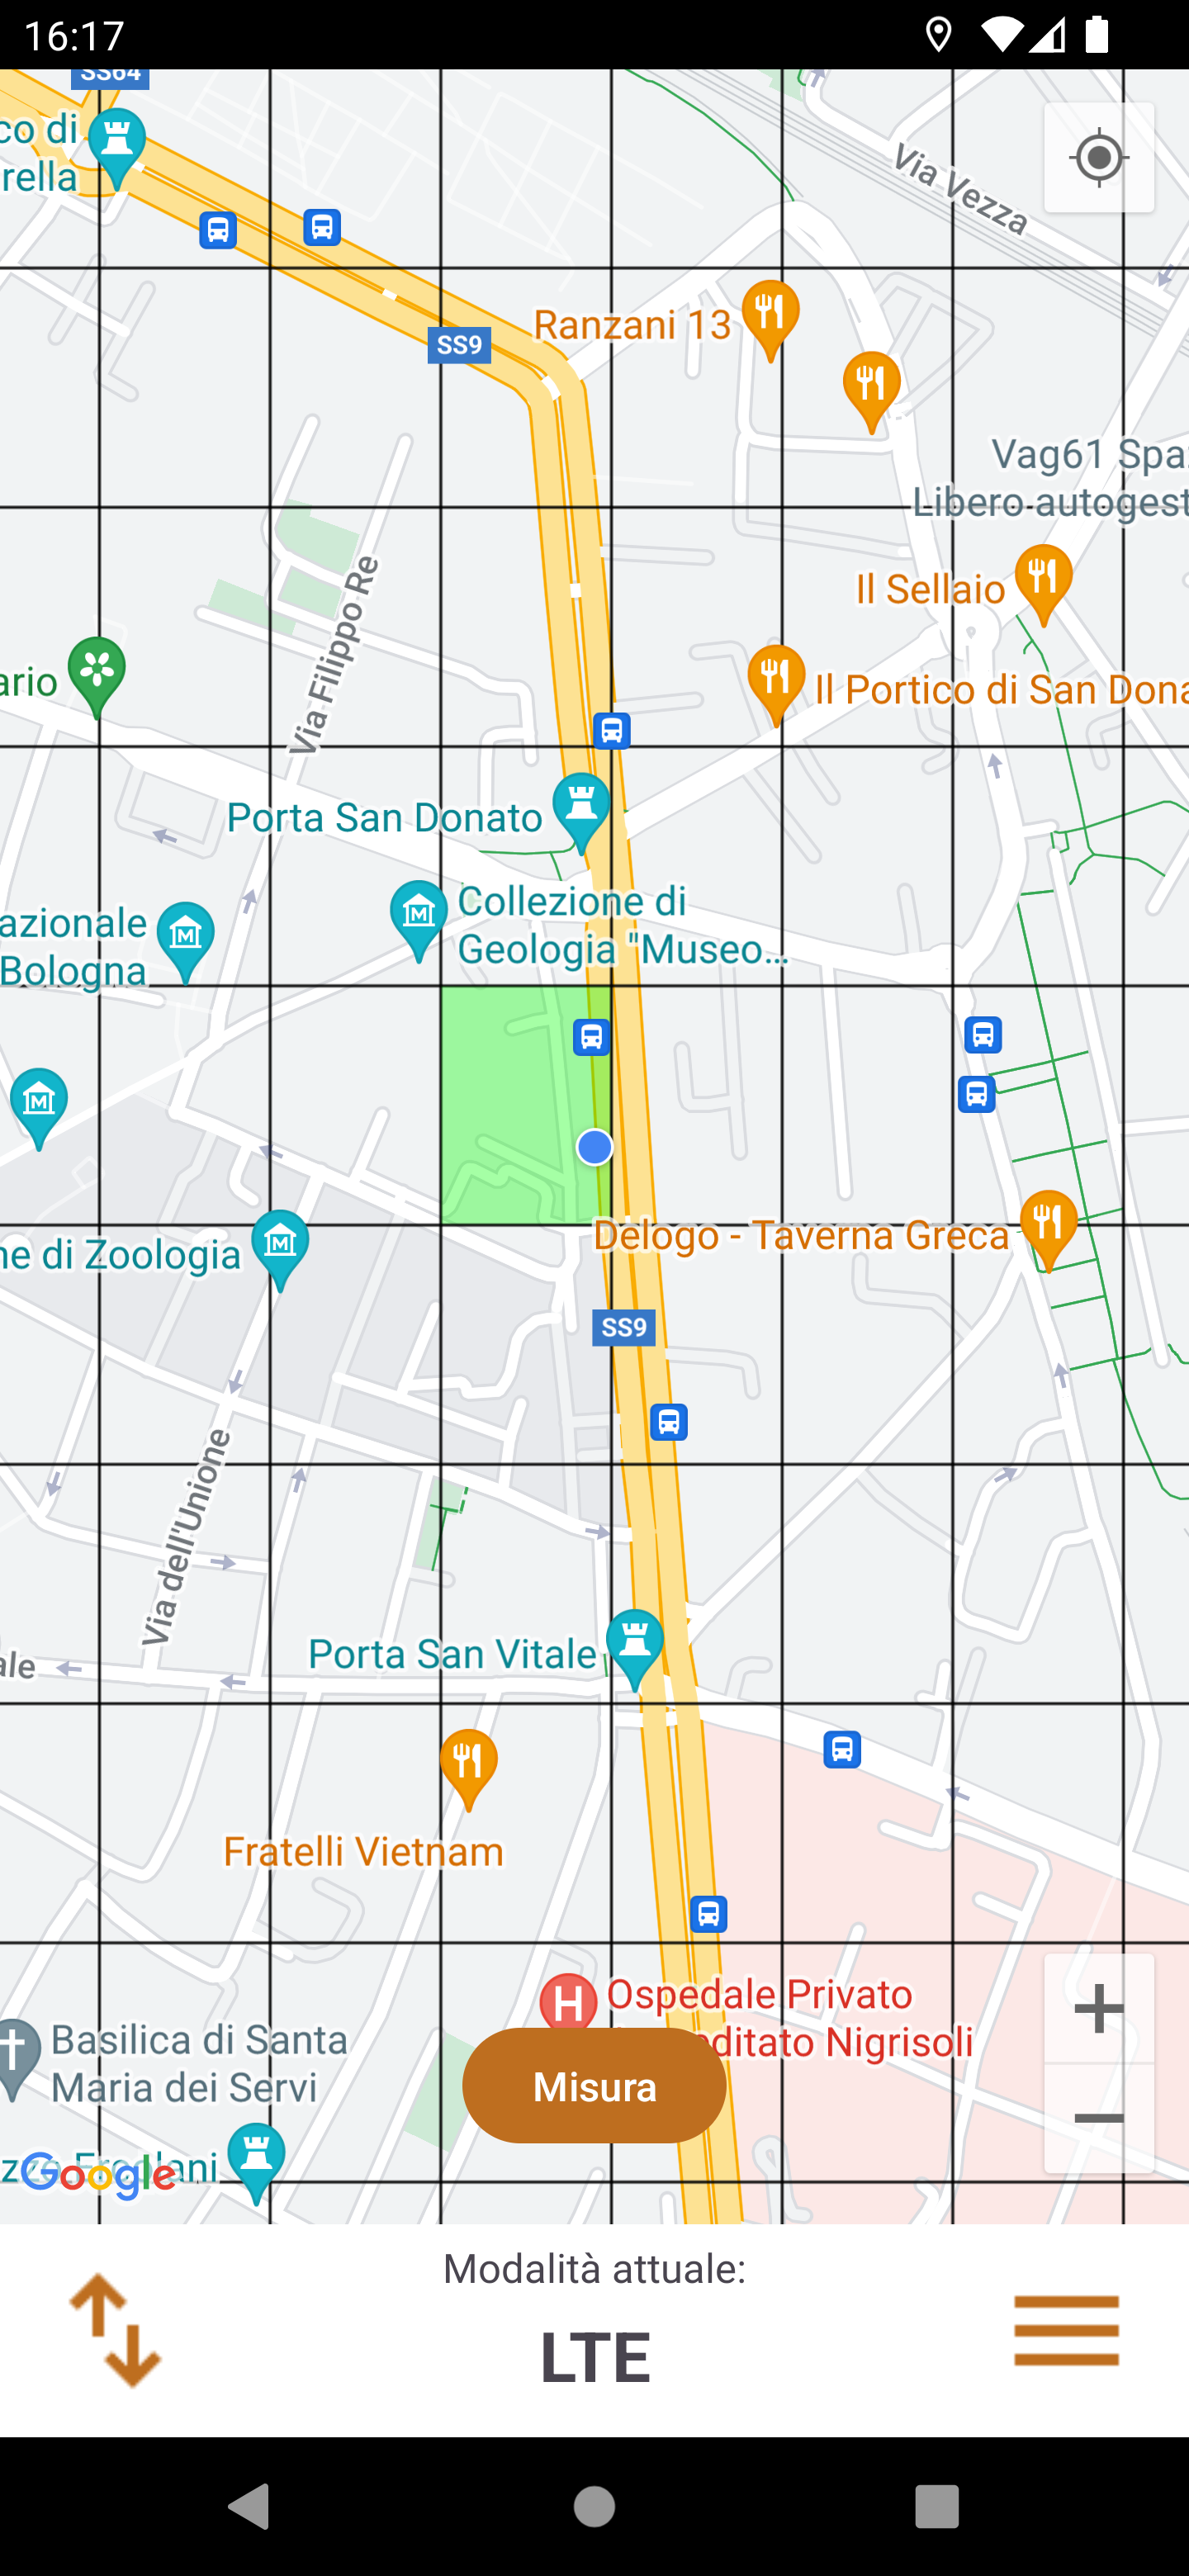
\includegraphics[width=\textwidth]{img/mainActivity.png}
        \caption{Schermata principale}
        \label{fig:mainActivity}
    \end{figure}
\end{minipage}
\begin{figure}[H] 
    \centering
    \subfloat[Premendo su un riquadro]{%
        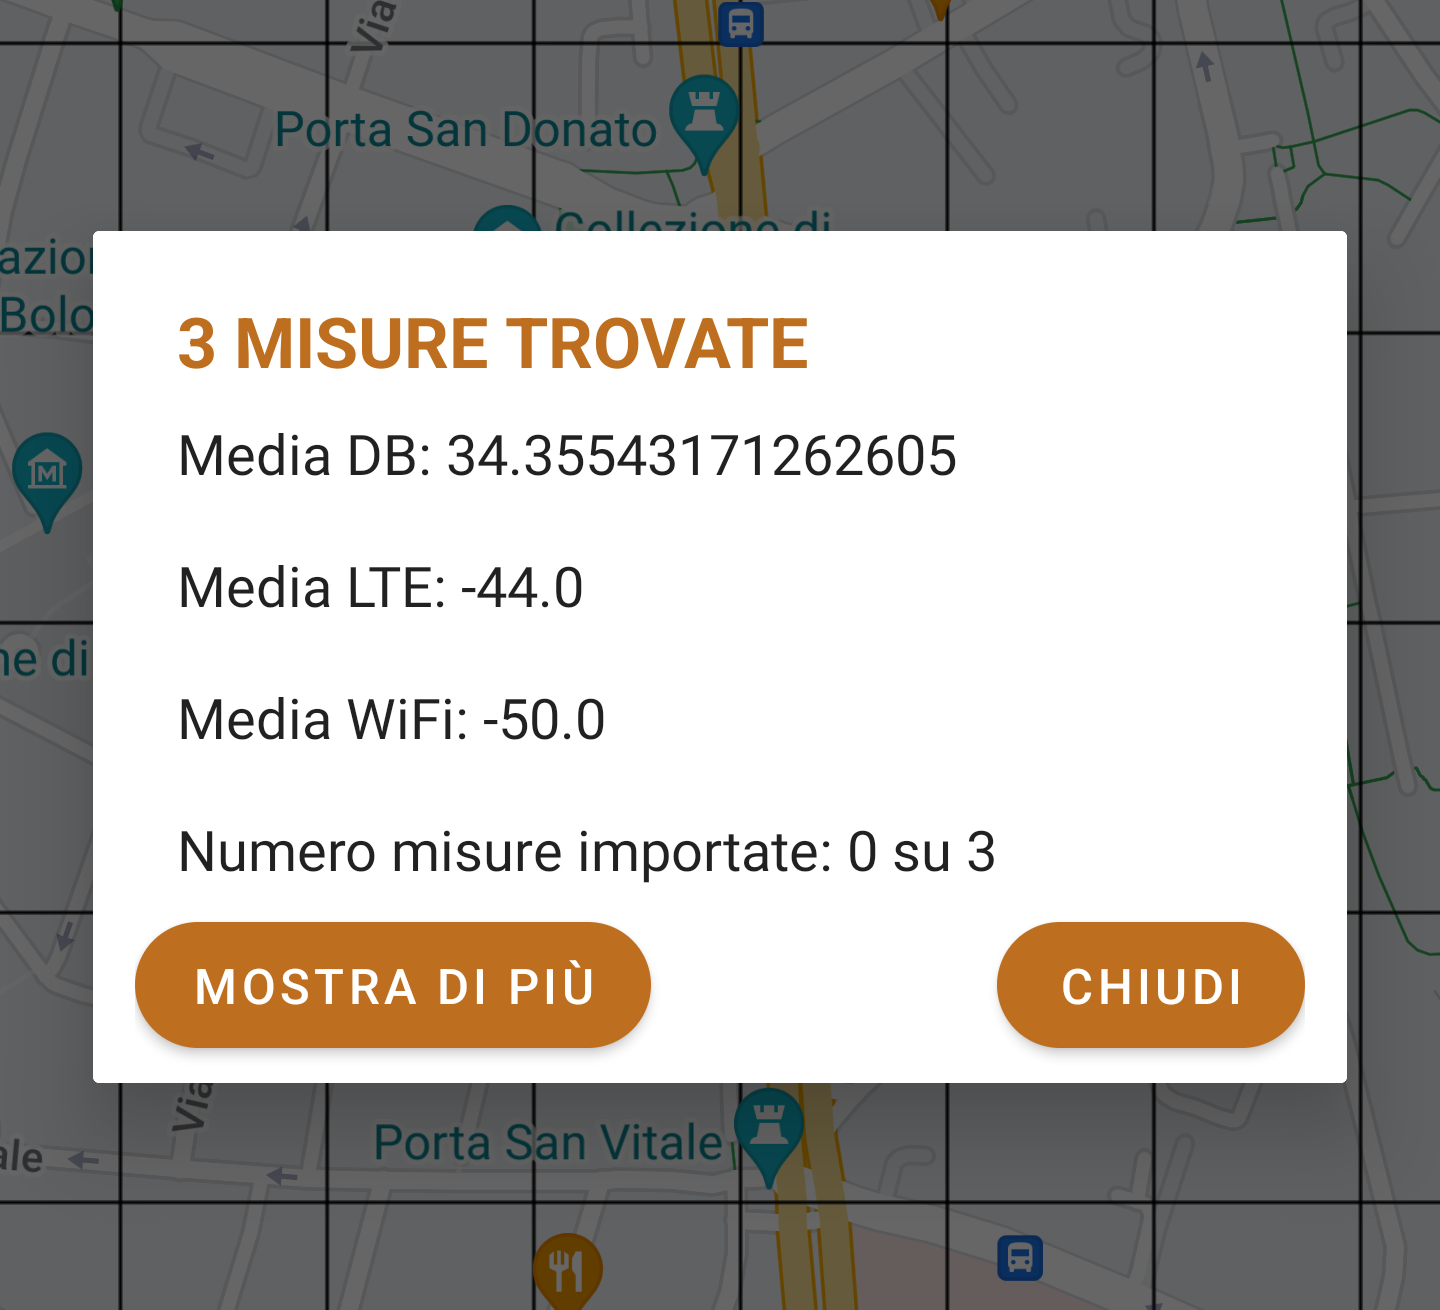
\includegraphics[width=0.3\textwidth]{img/showMore1.png}%
        \label{fig:showMore1}%
        }%
    \hfill%
    \subfloat[Premendo su "Mostra di più"]{%
        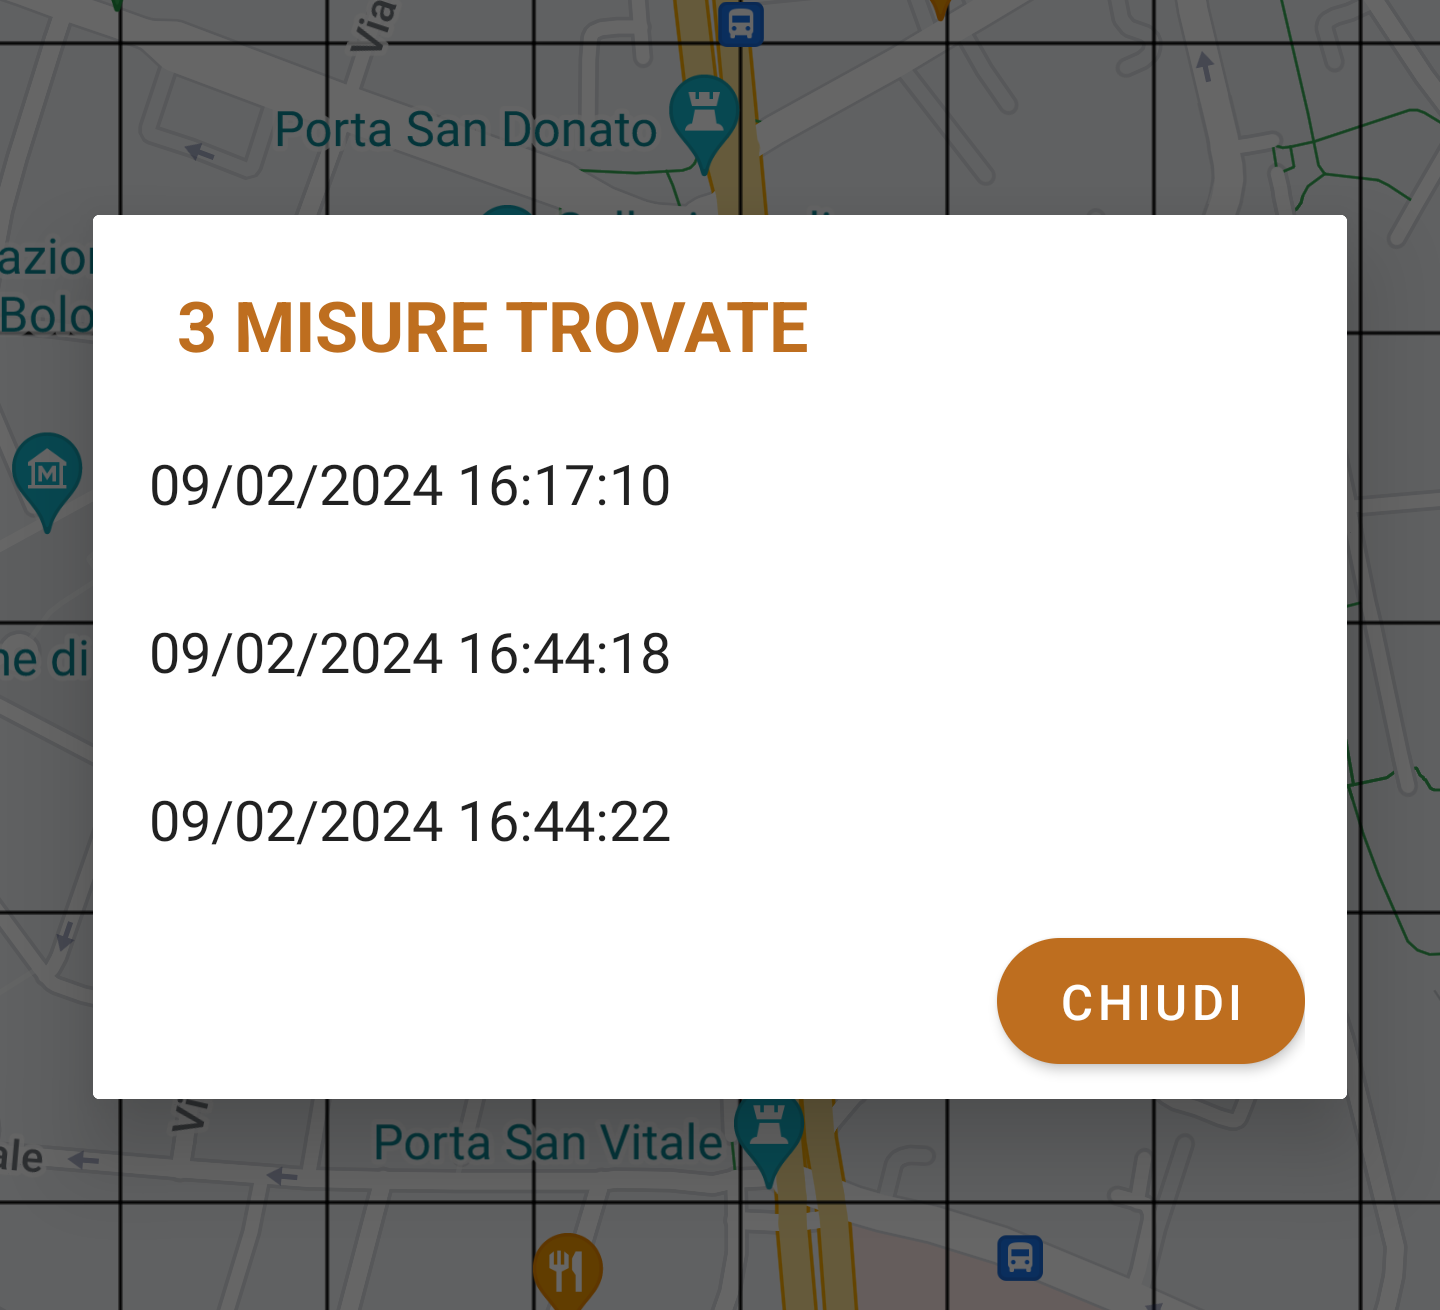
\includegraphics[width=0.3\textwidth]{img/showMore2.png}%
        \label{fig:showMore2}%
        }%
    \hfill%
    \subfloat[Premendo su una misura]{%
        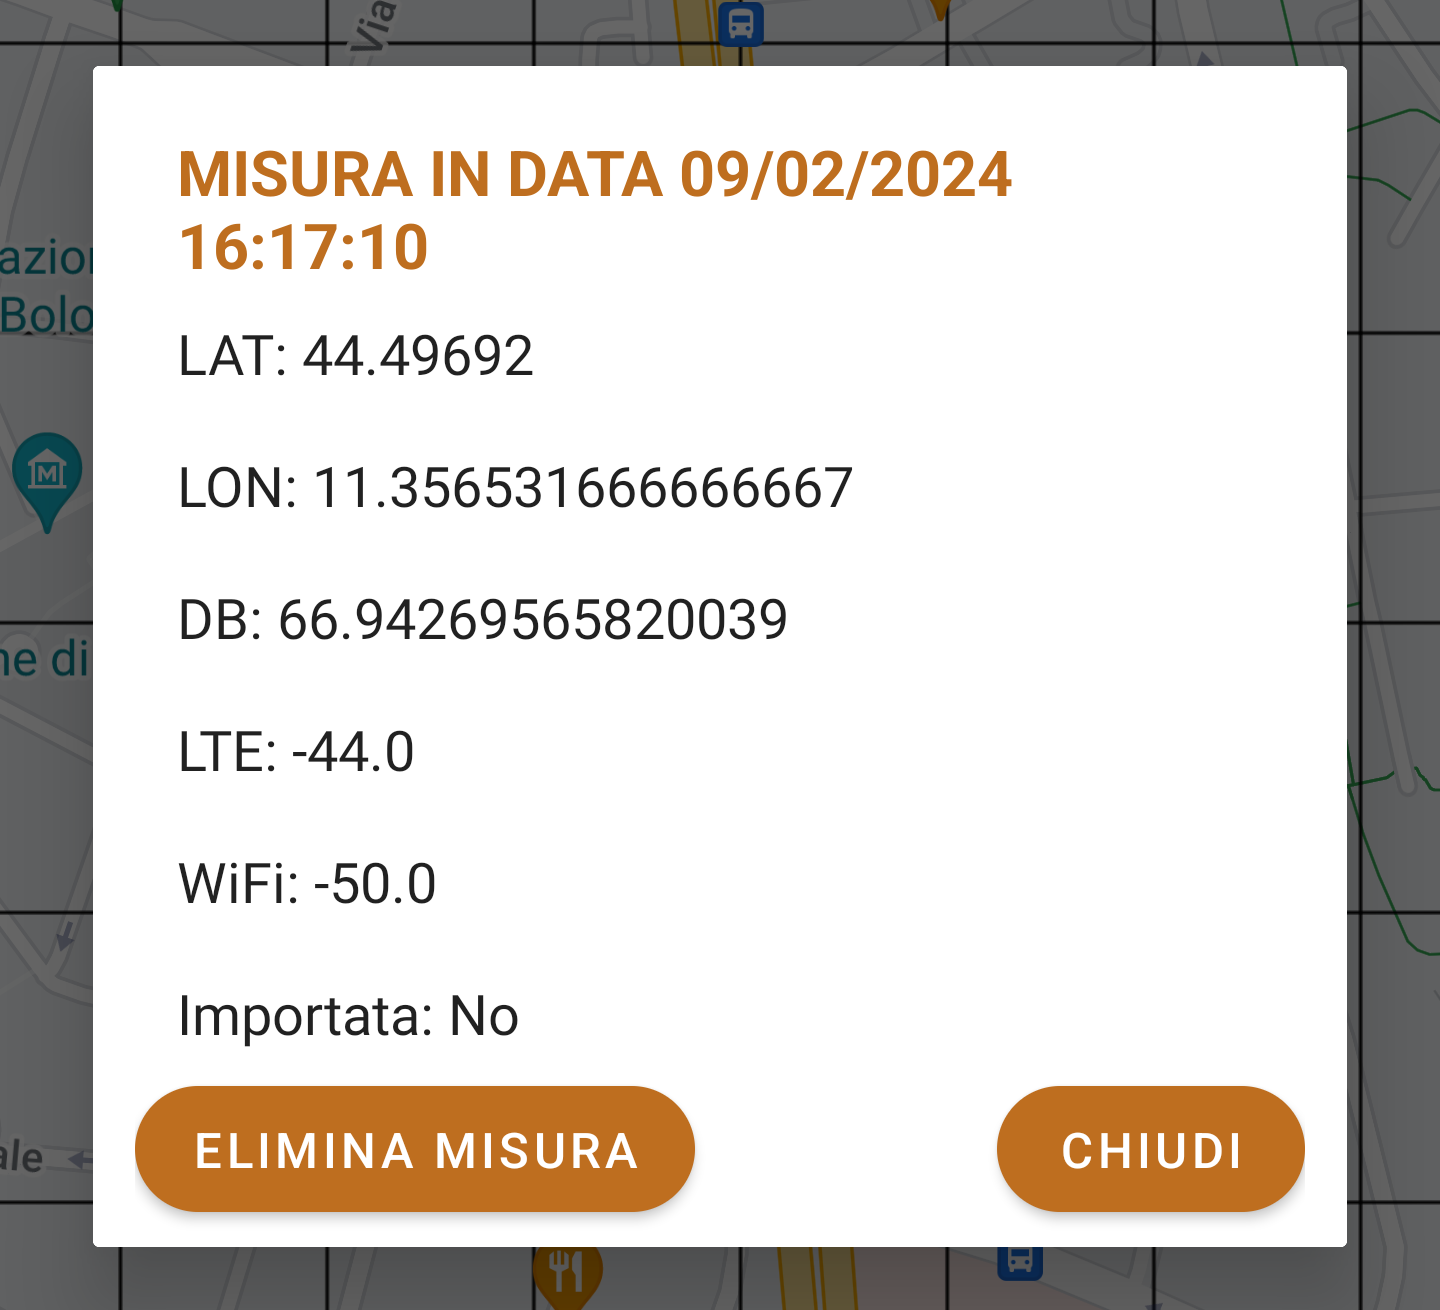
\includegraphics[width=0.3\textwidth]{img/showMore3.png}%
        \label{fig:showMore3}%
        }%

    \caption{Schermata riepilogativa}
\end{figure}
\pagebreak
\subsection{Settings Activity}
\label{sec:settingsActivity}
Schermata contenente tutte le impostazioni per le preferenze e modalità di misurazione. \\
L'utente ha la possibilità di scegliere:
\begin{itemize}
    \item Il tema, tra chiaro, scuro e predefinito del S.O.,
    \item Il parametro di visualizzazione, tra LTE, Wi-Fi o dB,
    \item Se mostrare o no le misure importate,
    \item Di attivare una particolare modalità di scansione, tra automatica, periodica e periodica in background,
    \item L'intervallo di scansione, ovvero ogni quanto effettuare una scansione quando è attiva quella periodica,
    \item La durata della discoverabilità, ovvero quanto rimanere discoverabile durante l'esportazione via Bluetooth,
    \item Di limitare le misure da tenere in considerazione da visualizzare sulla mappa e in caso affermativo ne può specificare il numero,
    \item Di impostare delle soglie manuali per la visualizzazione dei colori su mappa,
    \item Di attivare la funzionalità di notifica quando si entra in un riquadro con misure non recenti al giorno odierno,
    \item Di cancellare le misure (tutte, solo quelle effettuate dall'utente o solo quelle importate).
\end{itemize}
\begin{figure}[H] 
    \centering
    \subfloat[]{%
        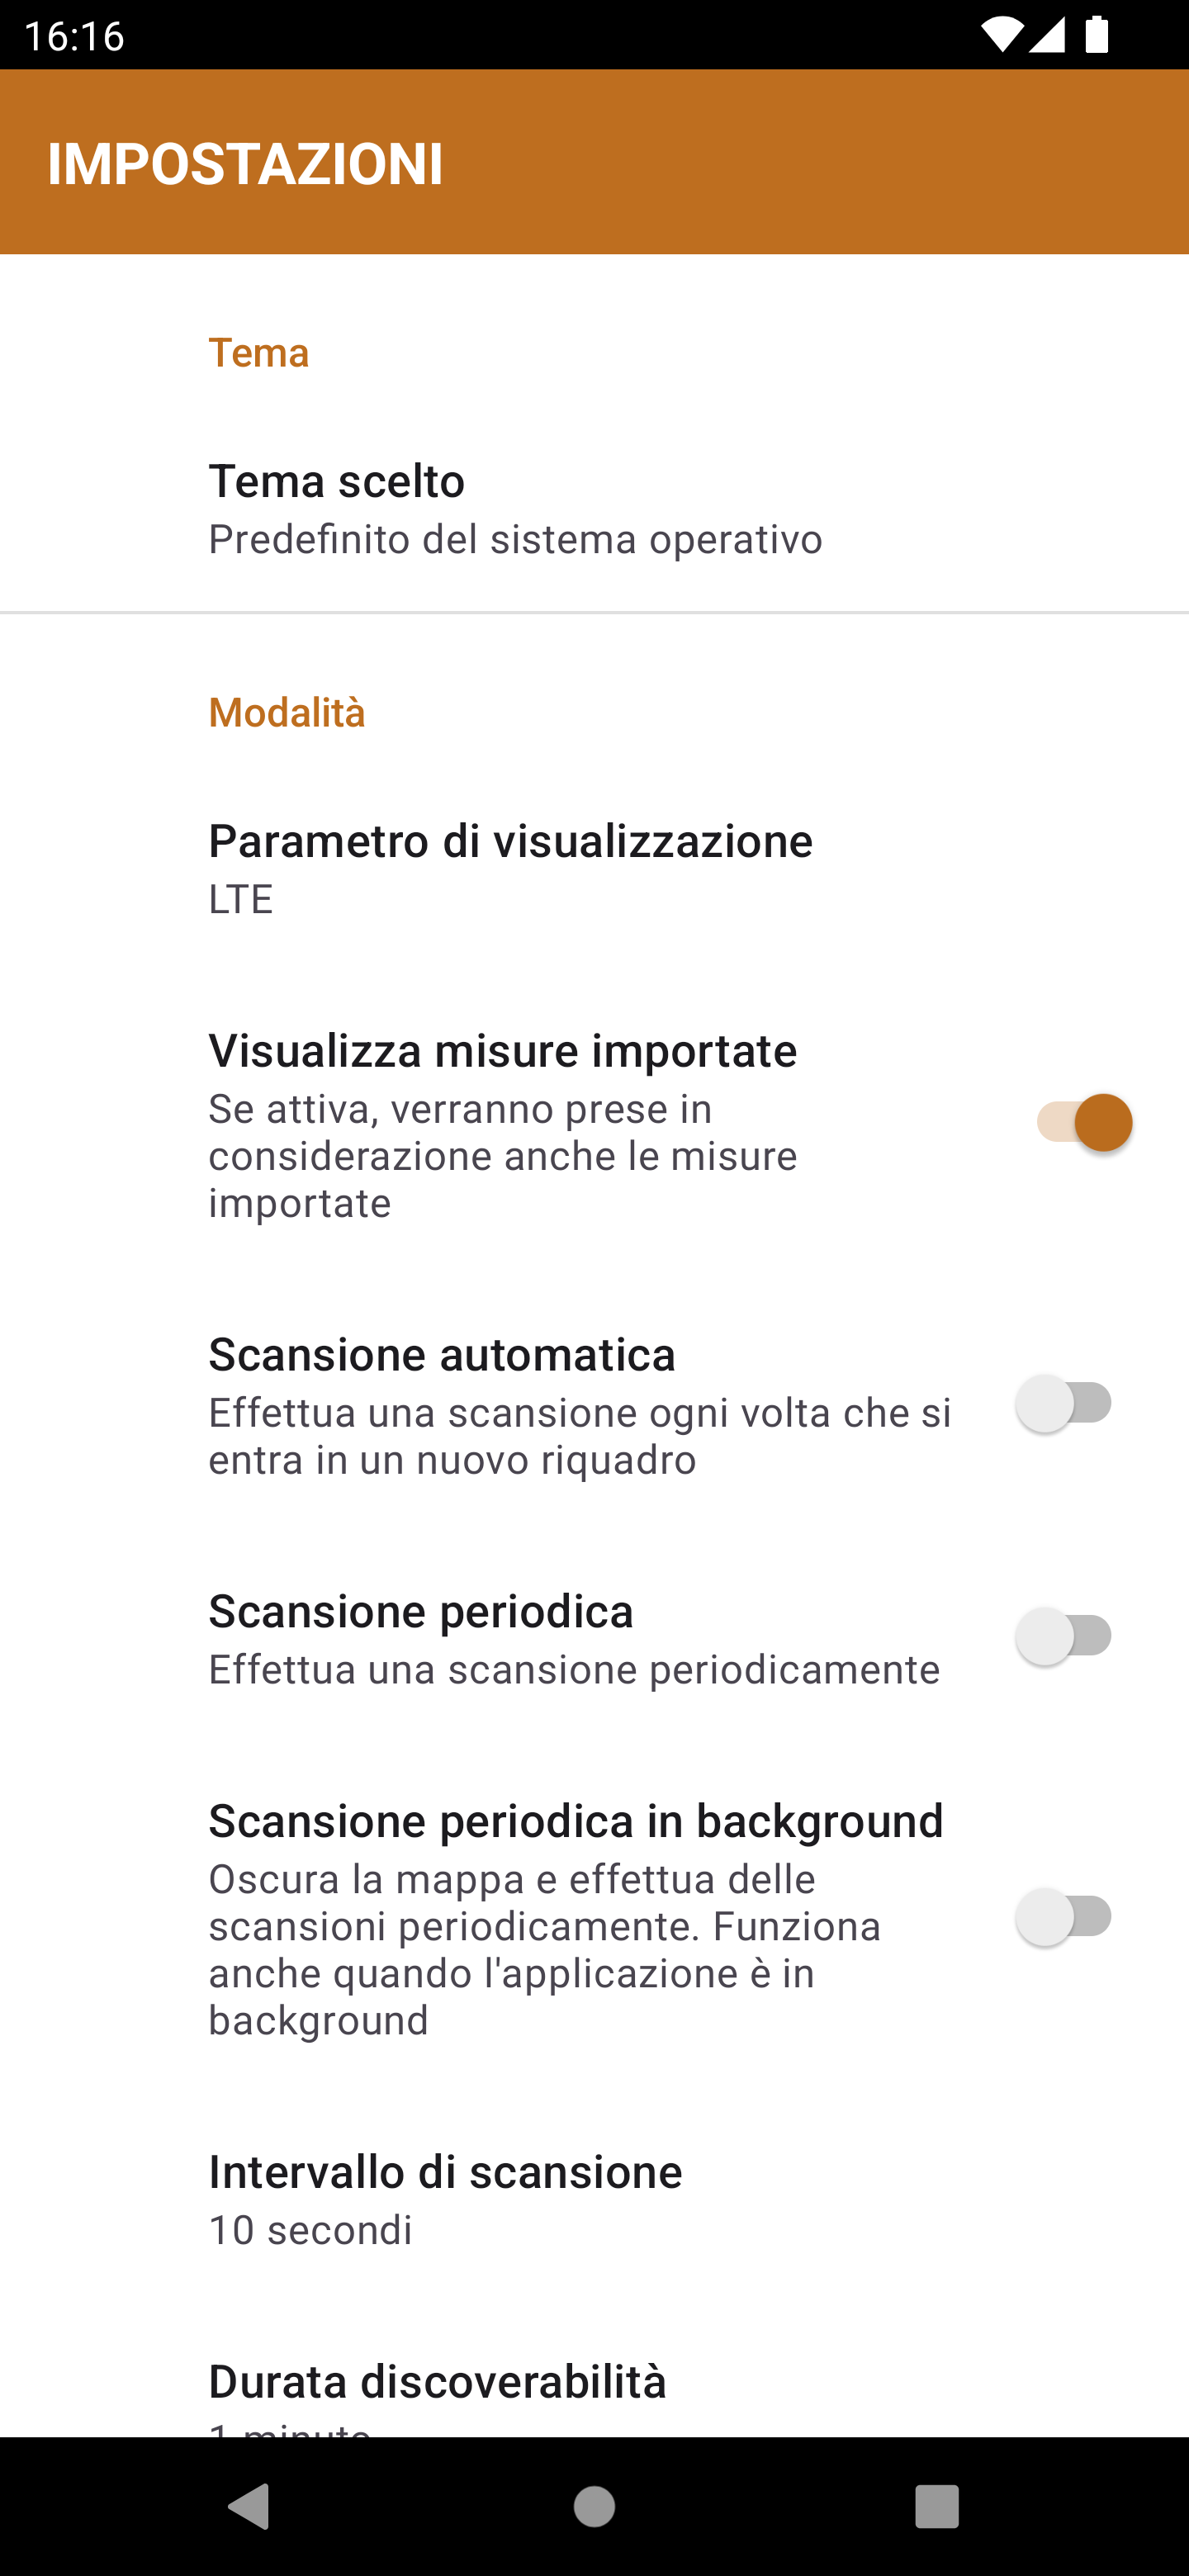
\includegraphics[width=0.3\textwidth]{img/settingsActivity1.png}%
        \label{fig:settingsActivity1}%
        }%
    \hfill%
    \subfloat[]{%
        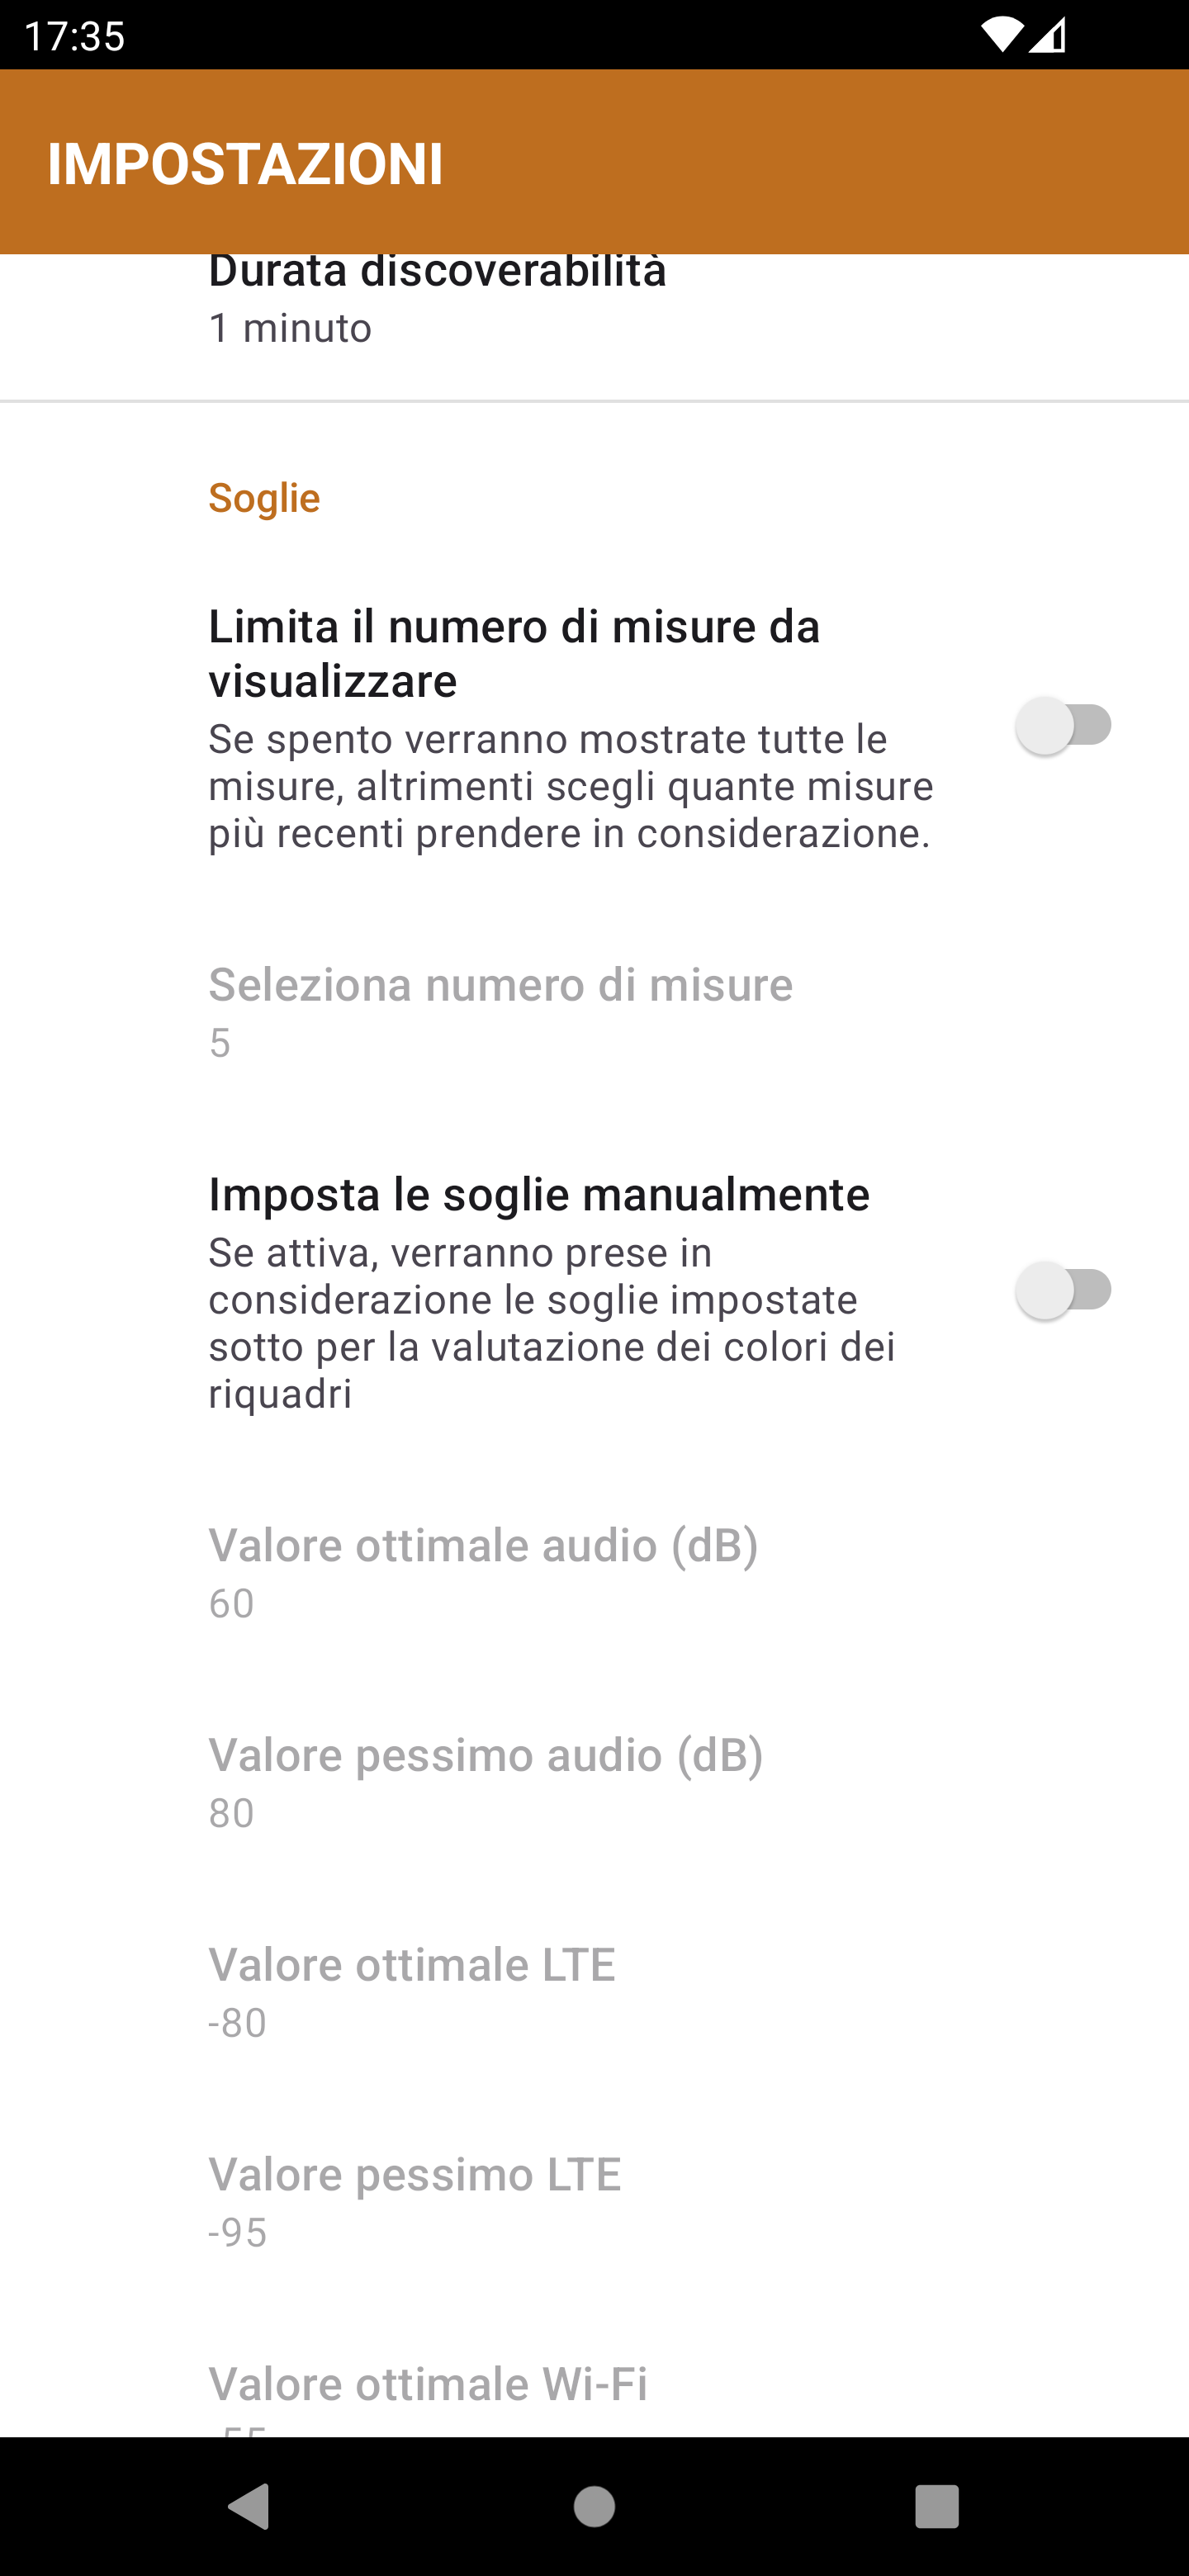
\includegraphics[width=0.3\textwidth]{img/settingsActivity2.png}%
        \label{fig:settingsActivity2}%
        }%
    \hfill%
    \subfloat[]{%
        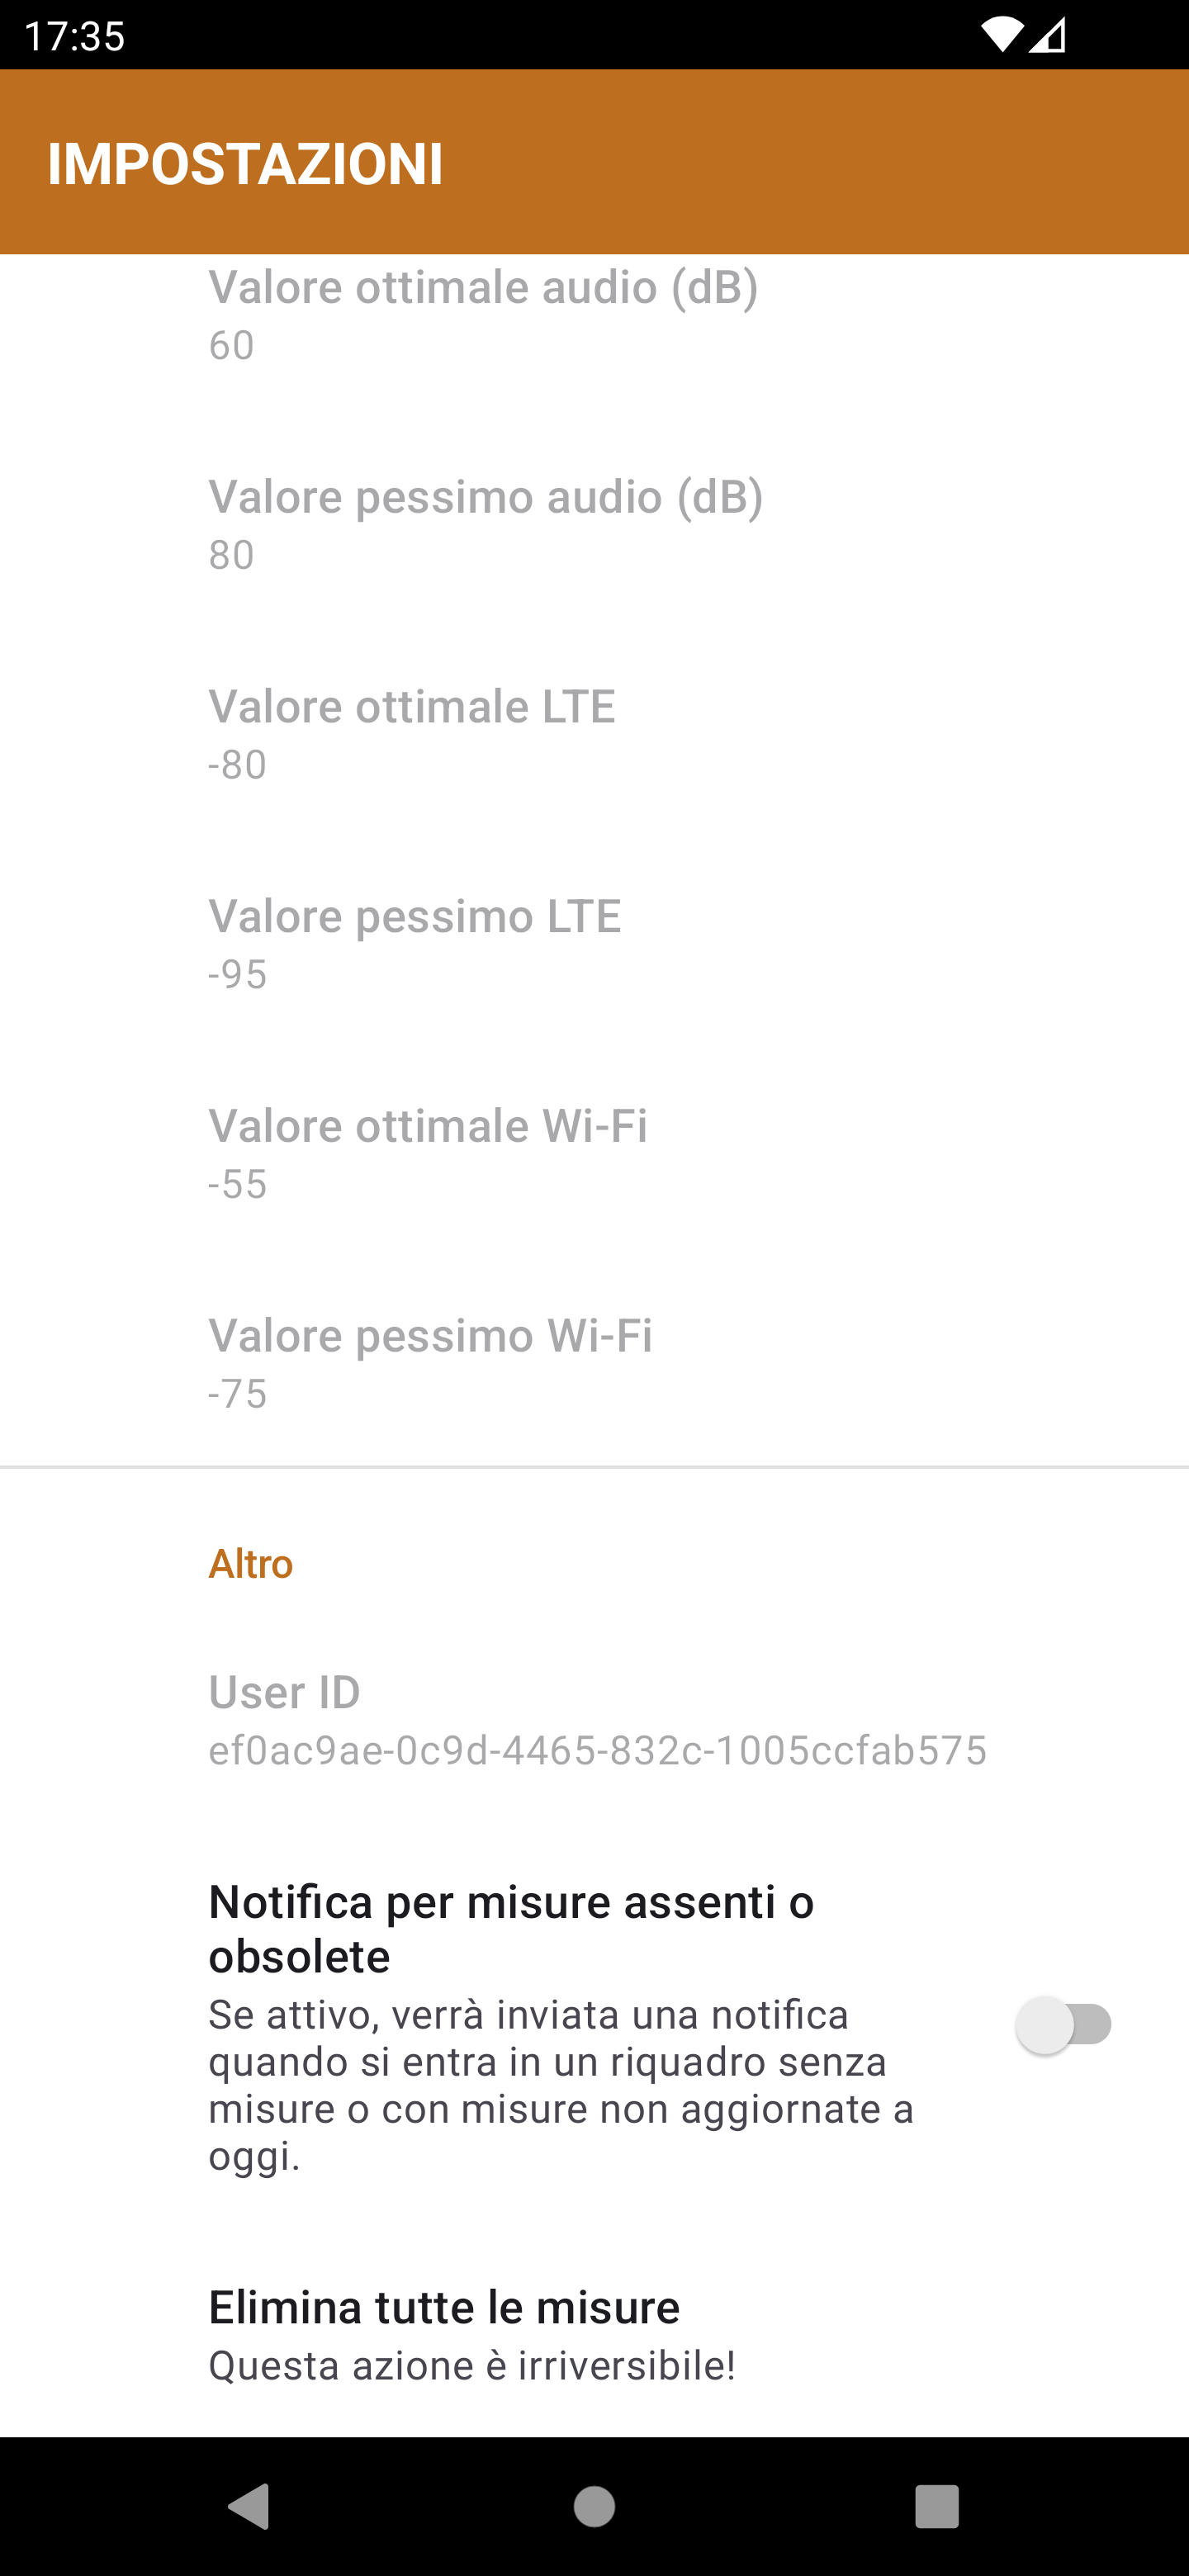
\includegraphics[width=0.3\textwidth]{img/settingsActivity3.png}%
        \label{fig:settingsActivity3}%
        }%

    \caption{Schermata delle impostazioni}
\end{figure}
\pagebreak
\subsection{Swap Activity}
\label{sec:swapActivity}
Schermata contenente le opzioni di scambio dati. \\
L'utente può scegliere di scambiare i dati con un altro dispositivo o tramite l'invio di file o tramite Bluetooth. \\
Ci sono quindi 4 opzioni:
\begin{itemize}
    \item Importazione da file: verrà chiesto di selezionare il file \texttt{.mapc} dall'archivio del dispositivo.
    \item Esportazione da file: verrà creato un file \texttt{export\_data-ora.mapc} contenente tutte le misure presenti nel database e verrà chiesto all'utente il modo di inviare tale file.
    \item Importazione da Bluetooth: verranno visualizzati i dispositivi nelle vicinanze discoverabili tramite Bluetooth e selezionandone uno verrà inizializzata la connessione per importare le misure automaticamente.
    \item Esportazione da Bluetooth: in base alla durata di discoverabilità presente nelle impostazioni, il dispositivo diventerà discoverabile dagli altri per quella durata e alla richiesta di importazione da parte di un dispositivo, gli invierà tutte le misure presenti nel database.
\end{itemize}
\begin{figure}[H] 
    \centering
    \subfloat[Schermata generale]{%
        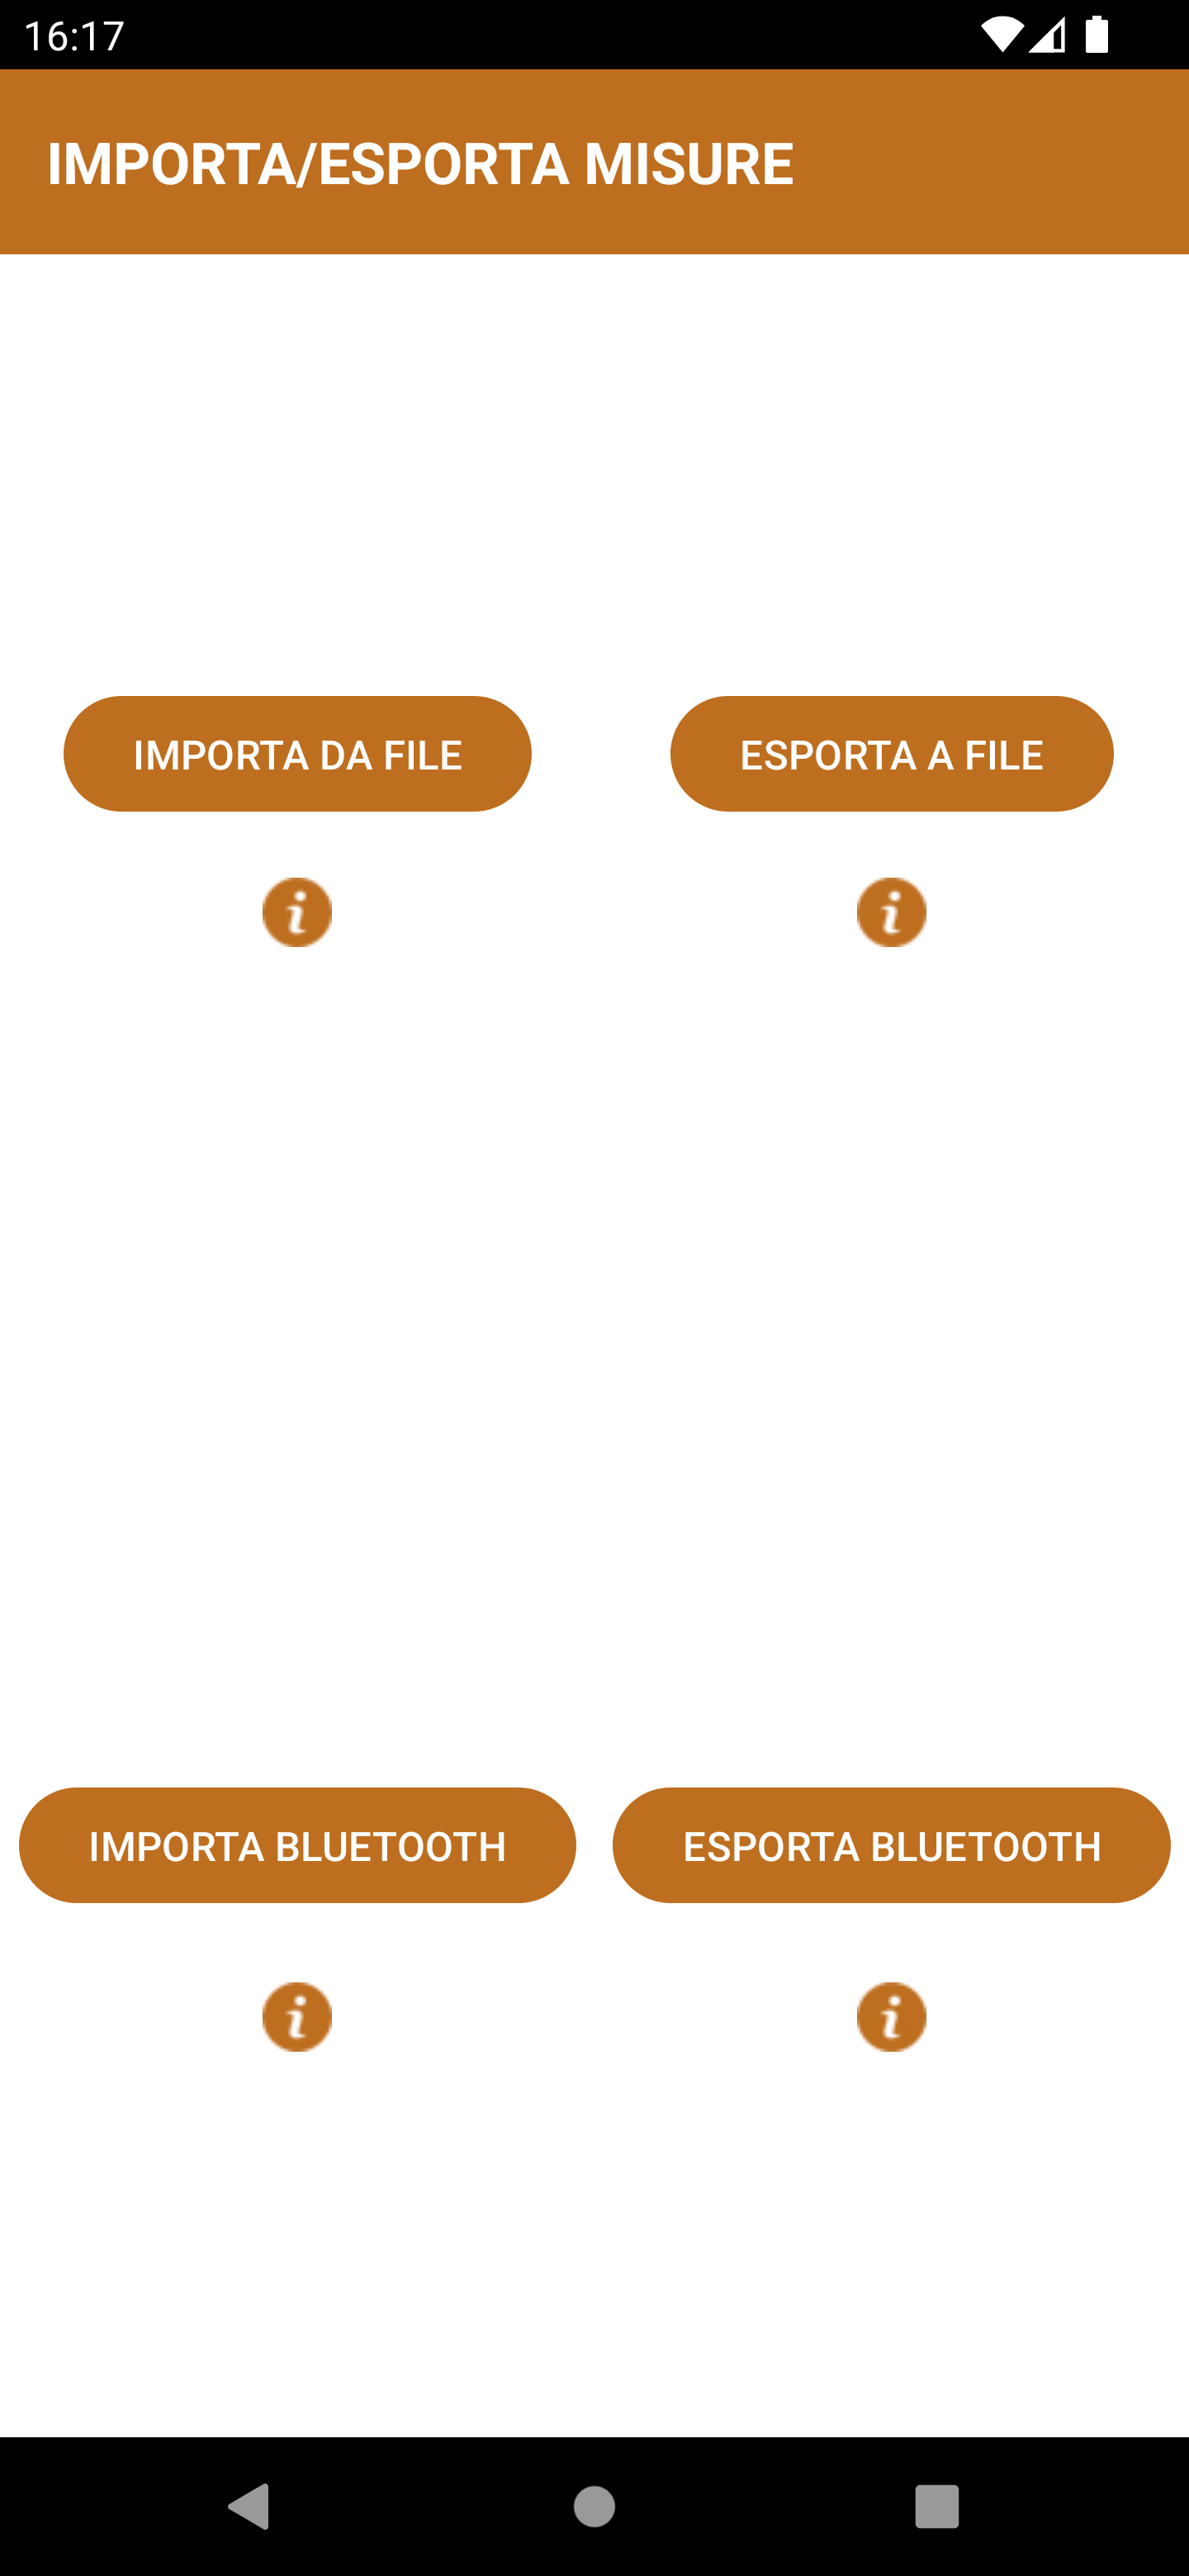
\includegraphics[width=0.3\textwidth]{img/swapActivity.png}%
        \label{fig:swapActivity}%
        }%
    \hfill%
    \subfloat[Schermata di importazione tramite Bluetooth]{%
        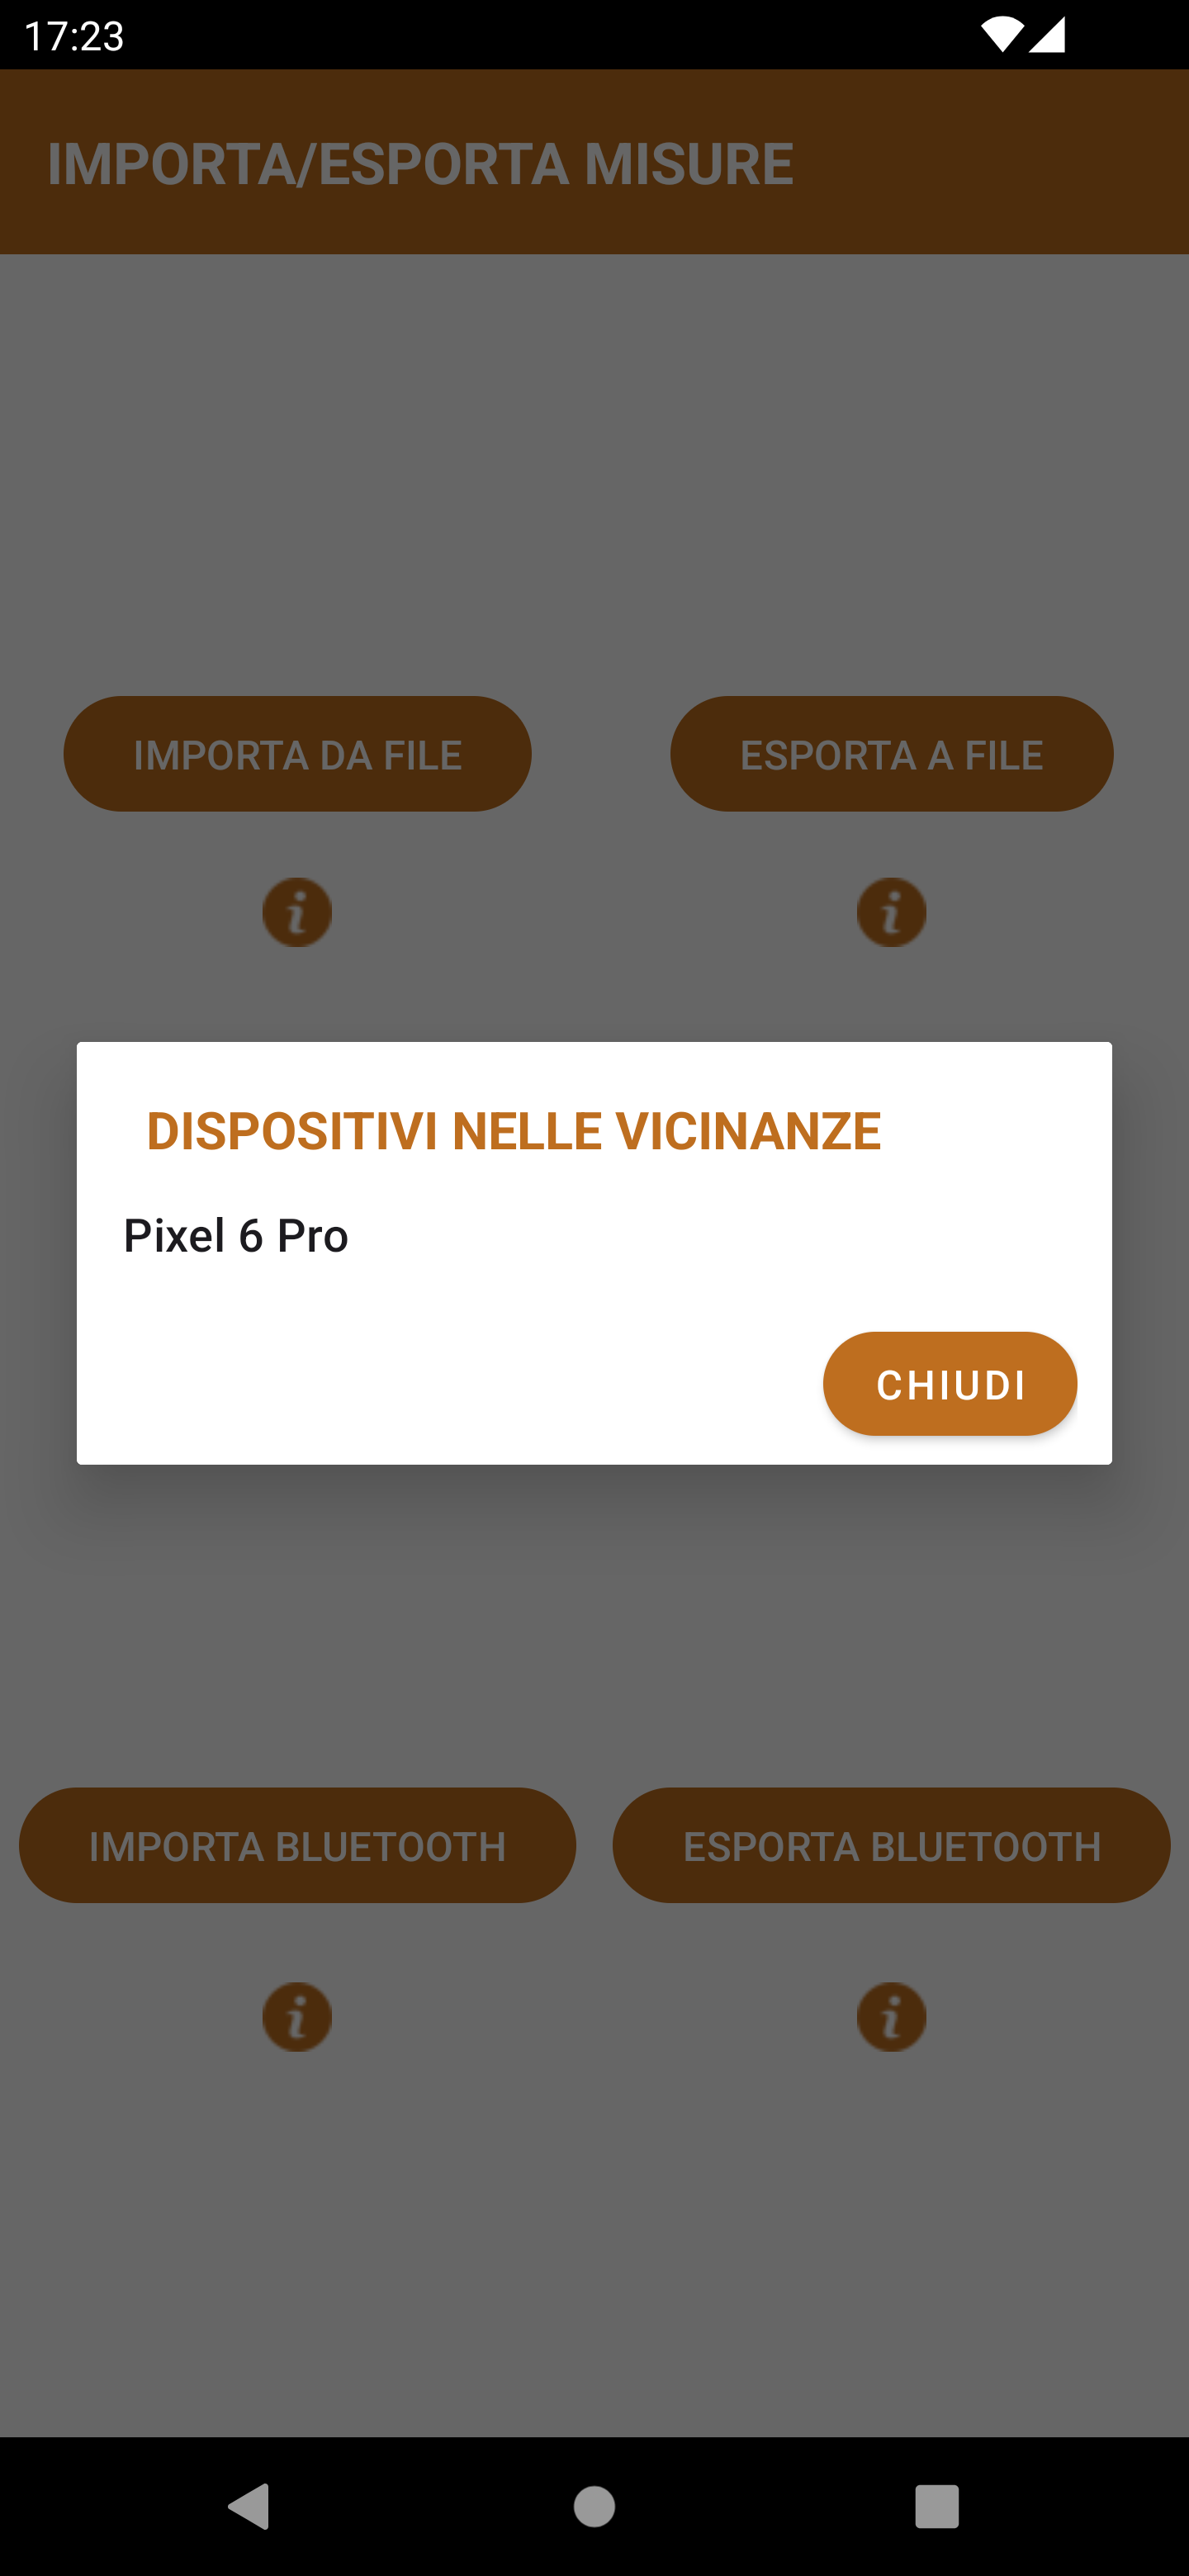
\includegraphics[width=0.3\textwidth]{img/importBluetooth.png}%
        \label{fig:importBluetooth}%
        }%
    \hfill%
    \subfloat[Schermata di esportazione tramite Bluetooth]{%
        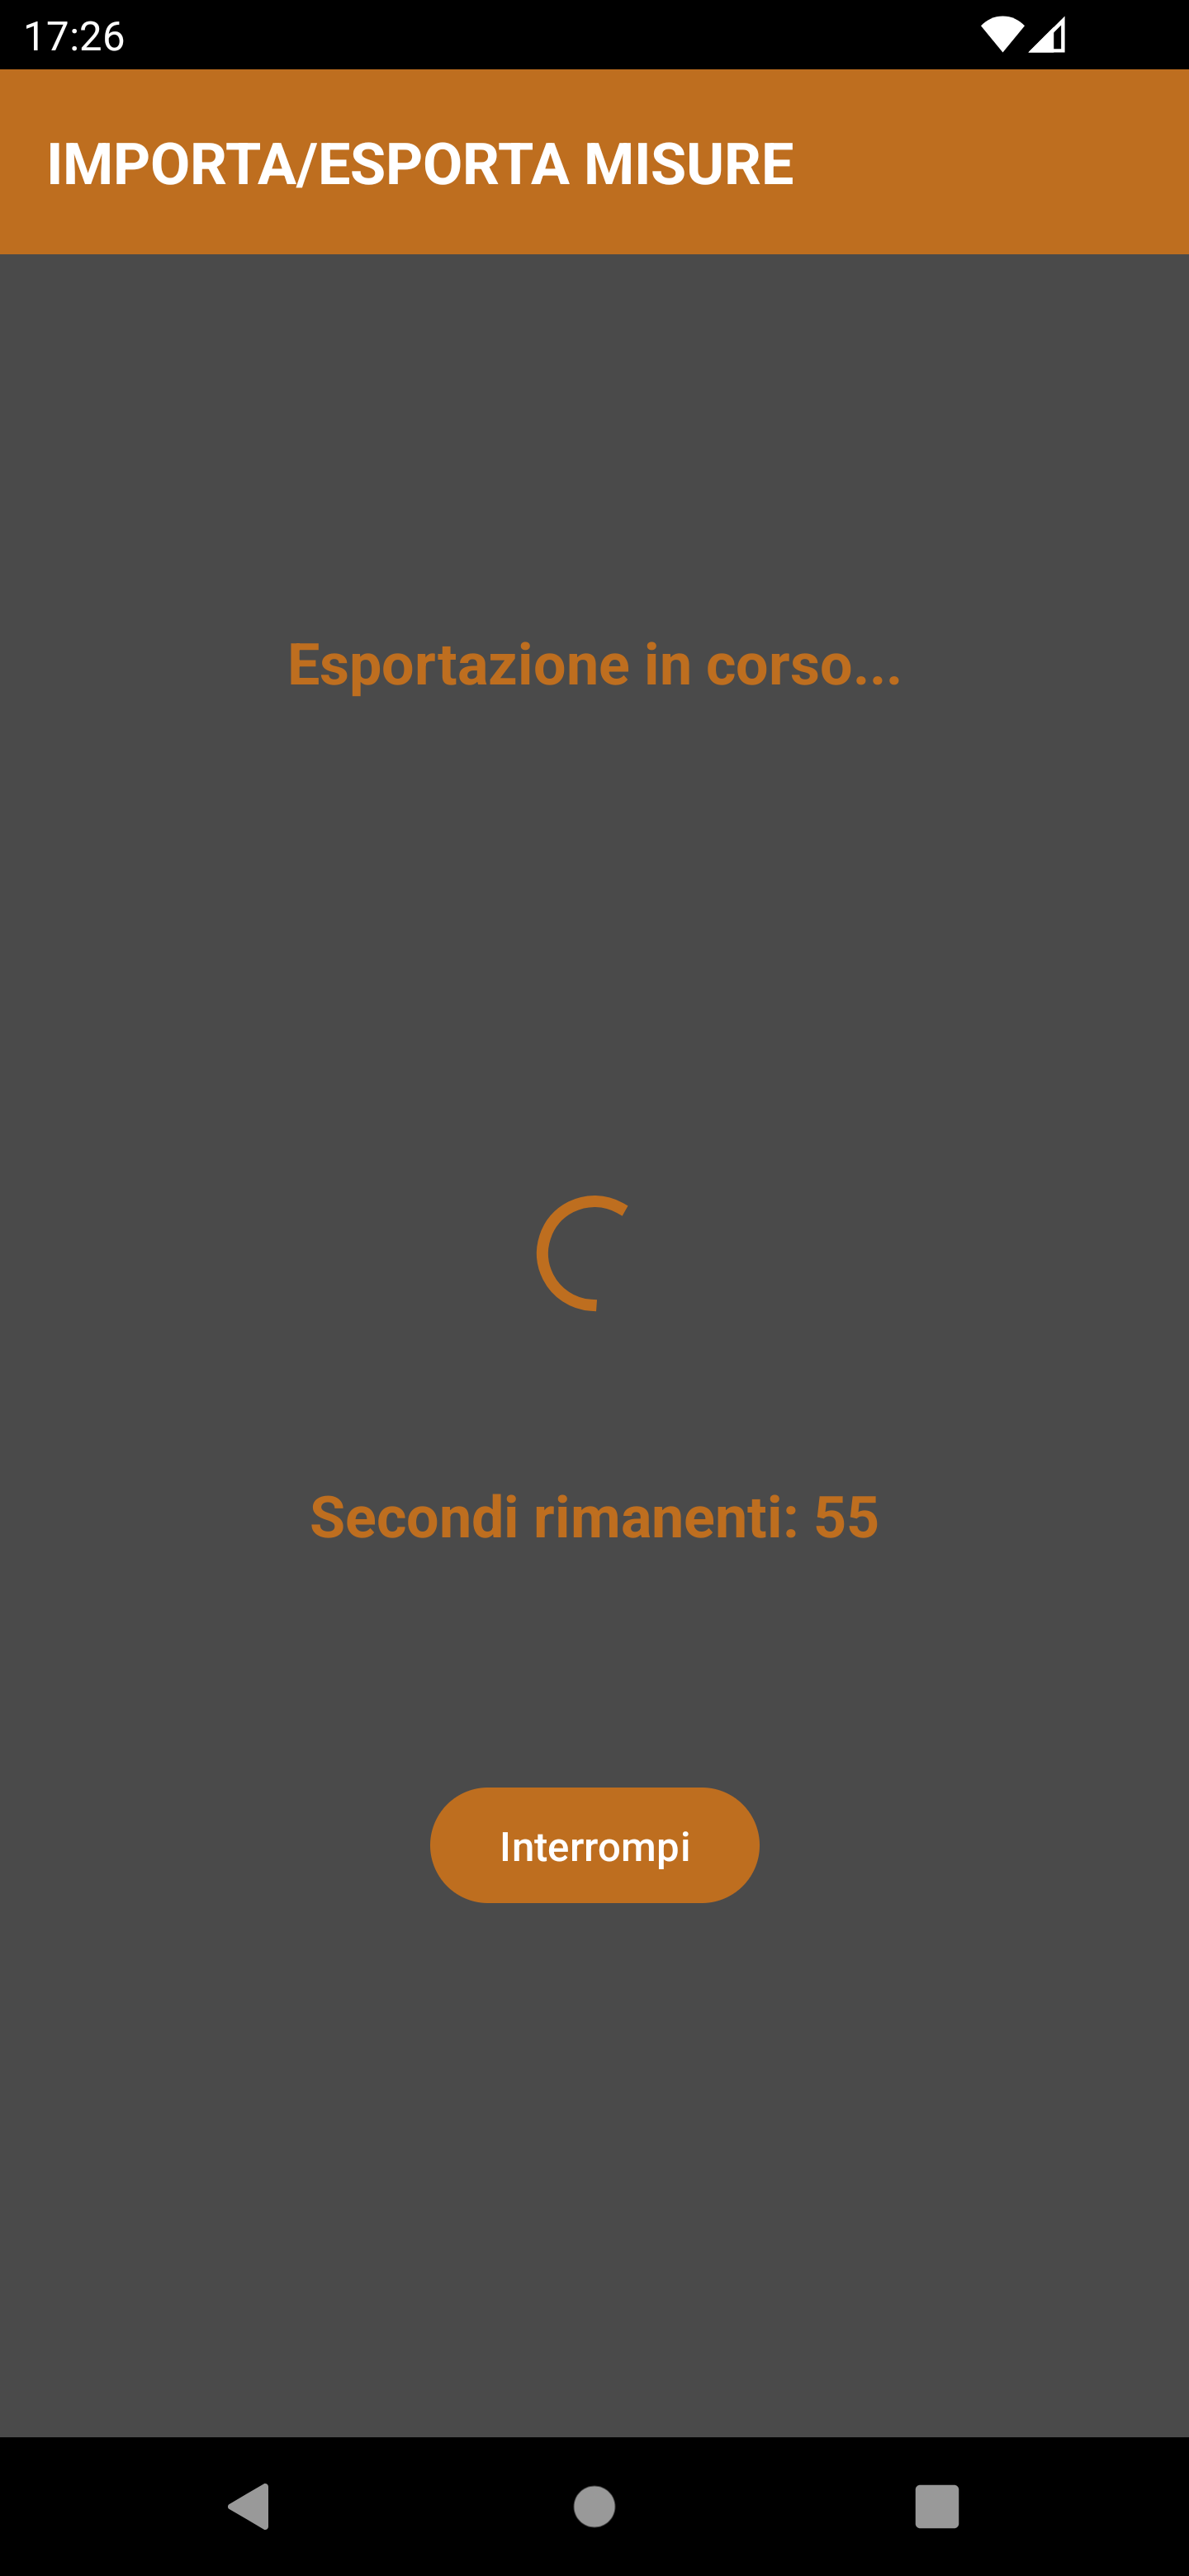
\includegraphics[width=0.3\textwidth]{img/exportBluetooth.png}%
        \label{fig:exportBluetooth}%
        }%

    \caption{Schermata di scambio dati}
\end{figure}
\section{Dettagli implementativi}
\subsection{Mappa}
Per la visualizzazione della mappa, sono utilizzate le \texttt{API} di \texttt{Google Maps} ed è implementata nella Main Activity tramite un fragment di classe \texttt{SupportMapFragment}. Viene inizializzata, tramite la funzione \texttt{loadMap}, dopo che l'utente ha fornito i permessi di posizione.
\subsubsection{Griglia}
\subsection{Sensori}
La gestione dei sensori avviene nella classe \texttt{Sensor} che implementa i metodi di misurazione per ciascuno dei tre componenti. \\
Le misurazioni LTE e Wi-Fi vengono effettuate instantaneamente, mentre per il calcolo del dB si campionano due misure del microfono nell'arco di tre secondi ignorando il primo perché non viene captato nulla. Una volta effettuato il campionamento, essendo calcolato in ampiezza, viene convertito in dB.
\subsection{Scambio di dati}
\subsubsection{Bluetooth}
\subsubsection{Da file}
\subsection{Metodi di misurazione} % Come effettua una misura, db ecc...
\subsubsection{Periodic}
\subsubsection{Periodic in background}
\subsubsection{Automatic}
\section{Capitolo 3 ex test effettuati}


\end{document}